\section{Variations on numerical parameters}
\label{sec:convergence}

The above halo-based metrics will have a certain level of dependence on the
choice of halo finder used. In an attempt to ensure independence of the
results from such factors, the above analysis was repeated  with the 3D
friends-of-friends (FoF) halo finder included in the {\tt yt} package
\citep{Turk2011}. We also repeated the analysis with the \velociraptor{} 6D
FoF finder \citep{Elahi2019}. The latter will disentangle active mergers, but
as active mergers make up a small fraction of the galaxy population, the
above results are qualitatively unaffected and only change quantitatively
to the 5\% level. The use of a FoF finder, rather than the spherical
overdensity finder found in AHF, did not qualitatively change the results.


In this section, we explore the implications of extending the Lagrangian
region of haloes while retaining the ability to capture non-uniform shapes. We
find that, in general, including more particles in the definition of the Lagrangian
region (than are present in the halo) leads to a fractionally higher level
of inter-Lagrangian transfer and more self-contribution to the final halo mass
at the expense of transfer from outside any Lagrangian region. This is expected, as
now many more particles are classified as being present in the Lagrangian region.


\subsection{Filling in Holes in Lagrangian Regions}


\begin{figure}
	\centering
	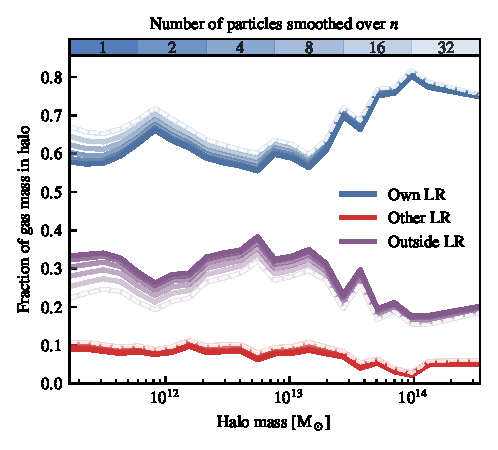
\includegraphics{figures/convergence_smoothing.pdf}
	\vspace{-0.7cm}
 \caption{The same as Fig. \ref{fig:maintransferresult}, but including
 Lagrangian region smoothing. Each line, coded by transparency, shows the
 fraction of gas mass in a halo from each component when the Lagrangian
 regions have been smoothed by 1 (i.e. the fiducial result), 2, 4, 8, 16, or
 32 particles (from darkest to lightest respectively). The white dashed line
 shows the result for the 32-smoothing case where the particles are given to
 the highest, rather than lowest, mass haloes; no difference is seen here
 suggesting that there is little overlap between the Lagrangian regions on
 these scales. See the text for the details of how this smoothing is
 constructed.}
	\label{fig:smoothconv}
\end{figure}

Our method for producing Lagrangian regions simply uses the dark matter
particles from a given halo; this naturally leads to a very diffuse
Lagrangian region. To see how the diffuse nature of these regions affects our
results, we smooth out the Lagrangian regions, by extending the procedure
that was used to extend the regions from the dark matter to the gas. This
works as follows:
\begin{enumerate}
	\item For every dark matter particle not in a Lagrangian region 
	      in the initial conditions, find the nearest $n$ neighbours.
	\item Find among the neighbours the maximal Lagrangian region ID,
	      corresponding to the lowest mass $z=0$ halo.
	\item Assign the particle the same Lagrangian region ID.
\end{enumerate}
The choice to assign the particles to the lowest mass halo, rather than the
higher mass halo, was made to ensure that spurious transfer into the lower mass
halo was avoided wherever possible. This means that the expectation is that
with this metric the level of inter-Lagrangian transfer will increase with
respect to the fiducial Lagrangian region identification method. This results
with the particles given to the haloes of a higher mass showing negligible
deviation from the fiducial result (see Fig \ref{fig:smoothconv}).


Note how smoothing the Lagrangian regions does have the expected effect of
inducing more inter-Lagrangian transfer, and does increase the proportion of
baryons that are classified as retained as the Lagrangian regions are filled
out. Despite this, the overall trends with respect to halo mass remain, with
a significant (>20\%) contribution from gas from outside Lagrangian regions
in haloes.

\subsection{The sizes of Lagrangian regions}

In Fig. \ref{fig:bigtransferpic} we saw that there was a large amount of
gaseous matter inside haloes from outside any Lagrangian region. It may be
reasonable to assume that this gas corresponds to dark matter that is simply
sitting just outside of the halo edge, perhaps within the so-called
`splashback radius'. The estimates for this radius range between 0.8 and
1.5$R_{\rm vir}$ \citep{More2015, Diemer2017a}, and hence below we consider
the situation where we extend the region around the halo that contributes to
the Lagrangian region. This is done in the following way:
\begin{enumerate}
	\item For every halo, find its current virial radius $R_{\rm vir}$. This contains
	      all particles at redshift $z=0$ that we consider to be within the halo.
    \item Now consider a new radius, $R_{\rm vir} \leq R_{\rm LR} \leq 1.5
		R_{\rm vir}$, and find all dark matter particles within this region
		from the halo centre. These dark matter particles are now defined to
		lie within the Lagrangian region of that halo.
    \item ID match these particles in the initial conditions to define the new
        Lagrangian region, extending to the gas in the usual way.
\end{enumerate}
\begin{figure}
    \centering
    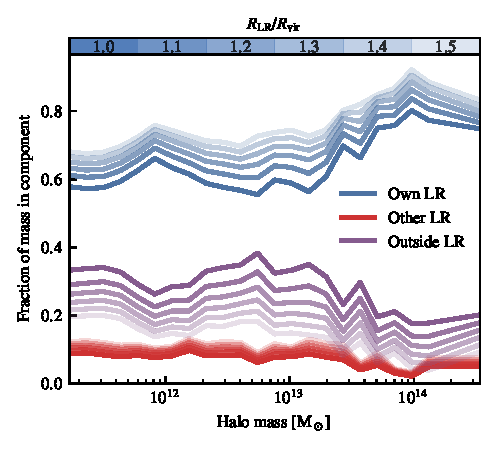
\includegraphics{figures/radius_convergence.pdf}
    \vspace{-0.7cm}
    \caption{The same as Fig. \ref{fig:maintransferresult}, but now showing
    how the Lagrangian make-up of haloes is changed with an increasing radius
    for the definition of the Lagrangian region. Lighter colours correspond
    to larger radii, going in steps of $0.1R_{\rm vir}$ from 1.0 to 1.5.}
    \label{fig:radius_dependence}
\end{figure}
The effects of this process on the gas component of Fig.
\ref{fig:maintransferresult} (where it is most significant) are shown in Fig.
\ref{fig:radius_dependence}.Here we see that there is a significant change in
the fraction of mass in the halo at redshift $z=0$ from outside any
Lagrangian region, especially when going to $R_{\rm LR} = 1.5 R_{\rm vir}$.
This large change is expected, though, as we now have included a volume that
is three times larger than the initial halo in the Lagrangian region
classification; taking this extreme value for all haloes really is a
`worst-case' scenario. The inter-Lagrangian transfer remains at a similar
level despite the increase in radius. Note that there will be no extra mass
included in the haloes here, with particles simply changing their Lagrangian
allegiances.

We chose this specific process, increasing the radius of our Lagrangian
region rather than the whole halo, to prevent us from simply re-defining our
halo size and including more gas as well (as in this case, the transfer
across the halo boundary would simply be moved to a larger radius). 